\chapter{State of the Art} \label{chap:sota}

This chapter presents a bibliographic review on the subjects covered by this project. Firstly, the concepts of Virtualization, Grid and Cloud Computing are presented, as well as a comparison between these two areas. There is also an analysis on existing developments, applications and projects on the area of Cloud and Grid Computing, with greater focus on two community driven projects (OpenStack and OpenNebula), since they are currently in use at FEUP. Some of the computing technologies in use at FEUP are also presented and discussed.

\section{Virtualization and Virtual Machines} \label{sec:virtualization} 

Throughout this project, Virtual Machines (VMs) are mentioned in great amount and as such, they deserve a special section.

Certain problems arise when the requirements of different virtual organizations (VOs) that need to use the same resources are in conflict or are incompatible with site policies. The software available on clusters cannot guarantee isolation of different communities and maintain resource availability while ensuring good utilization of those said resources. This is where Virtual Machines (VMs) come into play. They are emulations of lower layers of computer abstractions on behalf of the higher layers and allow the isolation of the applications from the hardware and neighbour VMs and customizing the platform so it suits the user's needs. \cite{clusters-grid, Zhang05virtualcluster} 

Virtualization benefits include an improvement in fault isolation and independence from guest VMs, performance isolation and simplifying the migration of VMs across different physical machines. These benefits enable VMs to share pools of platform and data center resources. \cite{virtualpower} 

The ability to serialize and migrate the state of a VM paves the way for better load balancing and improved reliability that cannot be achieved with traditional resources. Deploying virtual clusters - set of VMs configured to behave as a cluster and intended to be scheduled on a physical resource at the same time \cite{Zhang05virtualcluster} -  of diverse topologies requires the ability to deploy many VMs in a coordinated manner so that sharing of infrastructure, such as disks and networking, can be properly configured. This can become more costly than the deployment of single VMs.  

In order to understand more, it is necessary to define virtual workspaces (VWs). These are an aggregation of an execution environment and the resources allocated to that specific environment. It is described by the workspace metadata, containing all the information needed for deployment. An atomic workspace, representing a single execution environment, specifies the data that must be obtained and the deployment information that must be configured on deployment. It is also needed to specify a requested resource allocation, something that describes how much of each resource should be allocated to the workspace.

These atomic workspaces can then be combined to formed what is called a virtual cluster. Foster et al propose an aggregate workspace that contains one or more workspace sets - atomic workspaces with the same configuration. Cluster descriptions can be defined in ways that atomic workspaces can be constructed flexibly into more complex structures, organizing at the same time the infrastructure sharing between the virtual nodes. This deployment enables the user to specify different resource allocations for different members of aggregates defined like this. Foster et al consider that the trade-off they obtained is acceptable, as the slowdown suffered was of about 5\% and considering that virtual machines offer unprecedented flexibility in terms of matching clients to resources. \cite{clusters-grid}

Zhange et al also approached the virtual cluster theme in an article written with both Foster and Freeman, where they combine virtual clusters with Grid technology. The authors only considered two types of node within the cluster: head-nodes and worker nodes. They optimized the loading of the virtual images through image cloning (only transferring one image for all the worker nodes and one image for the head-node, therefore cloning all the worker node images at either staging or deployment time) and they considered that the cost of virtual cluster deployment and management is a good justification for expecting that they may be used for VOs for large groups of short jobs and single long-running jobs. They also found that the cost of running batch jobs in a a virtual cluster was very acceptable.\cite{Zhang05virtualcluster}

Katarzyna Keahey and Tim Freeman introduce the term \textit{contextualization} in order to describe the process of quickly deploying fully configured images and adapt them to their deployment context, for single VMs. The authors understand \textit{contextualization} as the process of adapting an appliance to its deployment context (an appliance defining an environment as an abstraction independent of its deployment). They are deployed dynamically and are potentially associated with a different context. According to the authors, they can also fulfill three different roles:
\begin{enumerate}
\item Appliance providers - they configure environments, maintain them and guarantee their consistency;
\item Resource providers - they provide resources with limited configuration requirements that are designed to support appliances but no longer to provide end-user environments for multiple communities;
\item Appliance deployers - they coordinate the mapping of appliances  onto available resource platforms and information exchange between groups of appliances to enable them to share information.\cite{contextualization}
\end{enumerate}

There are different types of approaches, since providers can have the applications running inside VMs or provide access to the VMs as a service (Amazon Elastic Compute Cloud), enabling the users to install their own applications. With virtualization, companies are trying to save power by getting the most of what they consume. Running several operating systems inside one machine, they can run independently and CPU idle time is kept to a minimum.\cite{aaron-clouds}

Virtualized computing clusters offer the advantage of being able to transform themselves to the user's needs. However, as pointed out by Nishimura et al, previous work has shown that the system does not scale when increasing the number of VMs and their detailed configuration is not allowed. To counter this issue, Nishimura et al propose a new way of managing virtual clusters so that a flexible and fully-customizable system integration by creating VMs on-the-fly is achieved. 

The authors also propose the creation of \textit{virtual disk caches} (VD caches), in order to reduce software installation time. This VD cache is created when a user requests it and is automatically destroyed to keep the total cache size within the given space. What the authors did was that when an installation request is made by the user, the system selects physical resources to host a virtual cluster for the request, instantiates a set of VMs and installs the operating system and other requested software to them. The experiments conducted by the authors using a prototype implementation showed that installing a 190-node virtual cluster can be done in 40 seconds, indicating that the installation of a 1000-VM could be done in under two minutes.\cite{nishimura}

Nathuji and Schwan addressed the issue of integrating power management mechanisms and policies with the virtualization techniques deployed in virtual environments. They propose the \textit{VirtualPower} approach which aims to control and synchronize the effects of the power management policies applied by the VMs to the virtualized resources. 

The authors propose this approach having in mind the current limitations in battery capacities and the power delivery and cooling limitations existent in data centers when they try to handle the constant demands of performance and scalability. The authors state that their approach  can exploit the hardware power scaling and the methods that control the power consumption of the underlying platforms. It takes guest VMs' power management policies and coordinates them through the system in order to achieve the objectives. 

The power management actions are encoded as a set of rules, these being based on a set of mechanisms which serve as a base to implement the power management methods. This approach aimed to present guest VMs with a set of power states and then use the state changes requested by the VMs as inputs to virtualization-level management policies, including those to use specific platforms and their power management capabilities, along with policies that take into consideration goals derived from the applications running through the whole system and from global constraints, such as rack-level limitations on maximum power consumption. 

Their findings showed that it is possible to respond to specific power management goals and policies implemented in guest VMs without a need for application specificity to be established at the virtualization level. \cite{virtualpower}

It is extremely important to discuss \textit{OpenNebula}, as this project will interact with it and as such, it is approached in a later section. \cite{opennebula}

\subsection{Hypervisors}\label{hyper}

An hypervisor is a piece of software that emulates the functioning of certain hardware, a process called \textit{Hardware Virtualization}. KVM - Kernel-based Virtual Machine - an open-source virtualization software\footnote{Nuno Cardoso compared XEN and KVM, but came to the conclusion that neither offered an advantage over the other, so KVM was chosen due to its simplistic installation process.} is used on the back-end of the project..

The following features for KVM were identified:
\begin{itemize}
\item Virtualization using hardware virtualization extensions, such as Inter-VT and AMD-V, thus enabling faster virtualization;
\item Symmetric Multi Processor emulation - enables multiprocessor hardware emulation;
\item Live migration of VMs between hosts, allowing VM relocation without downtime;
\item Paravirtualized networking and block devices, which enables faster emulation of those devices. \cite{nuno-cardoso}
\end{itemize}

\section{Grid Computing} \label{sec:grid}

Buyya et al believe that Grid computing facilitates the sharing, selection and aggregation of geographically dispersed resources, be it supercomputers, storage systems, data sources or even special assets owned by organizations for solving large-scale resource-intensive problems in different areas of expertise, and that was Grid computing's motivation.
Buyya also created a definition for "Grid" at the 2002 Grid Planet conference held in San Jose, United States:

\begin{quote}
	``A Grid is a type of parallel and distributed system that enables the sharing, selection, and aggregation of geographically distributed 'autonomous'
 resources dynamically at runtime depending on their availability, capability, performance, cost, and users' quality-of-service requirements.''\cite{Buyya2009599}
 \end{quote} 

Ian Foster, one of the most revisited authors regarding Grid computing, states that the “Grid” must be looked upon in respect of the applications it contains, the business value it generates and the scientific results it is capable of returning, instead of its architecture.
Carl Kesselman and Ian Foster wrote the following definition in their book ``The Grid: Blueprint for a New Computing Infrastructure'':
\begin{quote}
``A computational grid is a hardware and software infrastructure that provides dependable, consistent, pervasive and inexpensive access to high-end computational capabilities.''\cite{gridbook}
\end{quote}

Foster and Steve Tuecke redefined the definition, this time referring social and policy issues, affirming that Grid computing is related to resource sharing and problem solving in a coordinated manner and that these occur in dynamic, multi-institutional virtual organizations, the aspect to remember being the power to do something with the result. The authors also stated that they are preoccupied with the ``direct access to computers, software, data and other resources.''

As such, Foster proposes (as pointed out by the title of his article) a three point checklist that defines what a Grid system should be:
\begin{itemize}
\item The Grid should coordinate resources that are not subject to centralized control – Integration and coordination of both users and resources that live within different domains;
\item The Grid should use standard, open, general-purpose protocols and interfaces, as this will allow the establishment of dynamic resource-sharing arrangements and the creation of something more than an agglomerate of incompatible and non-interoperable distributed systems;
\item The Grid should deliver nontrivial qualities of service, such as response time, throughput, availability, security, co-allocation of multiple resource types to meet complex user demands, resulting in the utility of the combined system to be greater than just the sum of its parts.
\end{itemize}

Foster also states that the Web is not a Grid, as though its general-purpose protocols support the access to distributed resources; they do not coordinate their use to deliver qualities of service.

Some large-scale Grid deployments inside the scientific community abide by the three points described by Foster, such as NASA’s Information Power Grid and the TeraGrid, which will link major U.S. academic sites, as they integrate resources from several institutions, use open and general-purpose protocols (Globus Toolkit, which will be discussed in further details later on this report) to negotiate and manage sharing and they address multiple dimensions of the quality of service, such as security, reliability and performance.\cite{Foster_2002}

Stockinger started a survey where he contacted over 170 Grid researchers globally spread in order to obtain a general feel on how the Grid was being defined. The results showed that the Grid infrastructure should provide a set of capabilities, such as:
\begin{itemize}
\item Description of available resources, what they are capable of doing and how they are connected;
\item Visibility into the state of resources, including notifications and logging of significant events  and state transitions;
\item Assurance of the quality of service across an entire set of resources for the lifetime of their use by an application;
\item Provision, life-cycle management and decommissioning of allocated resources;
\item Accounting and auditing of the service;
\item Security.
\end{itemize}

The results also showed that a Grid should have a set of characteristics, including:
\begin{itemize}
\item Collaboration - sharing resources in a distributed manner;
\item Aggregation - the Grid is more than just the sum of all parts;
\item Virtualization - Services are provided in a way that the complexity of the infrastructures is hidden from the end-user through the creation of an abstract "layer" between clients and resources;
\item Heterogeneity;
\item Decentralized control, Standardization and Interoperability - supporting Ian Foster's definition;
\item Access transparency - users should be able to access the infrastructure without having to preoccupy themselves how they are doing it;
\item Scalability; 
\item Reconfigurability;
\item Security - specially since the systems are often spread through multiple administrative domains. \cite{stockinger}
\end{itemize}

The members of the EGEE (Enabling Grids for E-sciencE Project) also state that their Grid abides by some of the characteristics mentioned above, namely "decentralized control", "heterogeneity" and "collaboration" \cite{grids-and-clouds}. Their Grid is described in greater detail in the "Grids VS Clouds" section below. 

Bote-Lorenzo et al also identified some core Grid characteristics that coincide with Stockinger and Ian Foster's definitions. These include scalability, heterogeneity, resource coordination and dependable, consistent and pervasive access. The propose the following definition for a Grid:

\begin{quote}
``... large scale geographically distributed hardware and software infra-structure composed of heterogeneous networked resources owned and shared by multiple administrative organizations which are coordinated to provide transparent, dependable, pervasive and consistent computing support to a wide range of applications. these applications can perform either distributed computing, hight throughput computing, on-demand computing, data-intensive computing, [...]''\cite{bote-lorenzo}
\end{quote}

Baker et al say that the Grid has evolved from something static and carefully configured, to what has been witnessed in the past years, where it became a seamless and dynamic virtual environment, capturing the attention from the industry and thus making an impact on the Grid's architecture and protocols and standards. 

The authors also describe a few standards and organizations that have been actively present in the Grid's environment over the past years. These include the Global Grid Forum (GGF), a community-driven set of groups which goal is to develop standards and best practices for wide-area distributed computing. The GGF creates a group of documents that provide some information to the Grid community, dividing its efforts into several categories, including architecture, data and security.

The authors also approach the World Wide Web Consortium (W3C), an international organization created to promote common and interoperable protocols. This organization was responsible for creating the first Web Services specifications in 2003, such as SOAP and the Web Services Description Language (WSDL).
According to the authors, the most important Grid standard to appear recently is the Open Grid Services Architecture (OGSA), which goal is to define a common, standard, and open architecture for Grid-based applications. It was announced by the GGF at the Global Grid Forum in 2002 and in March 2004 it was declared by the GGF to be the flagship architecture.\cite{grid-standards}

Iosup, Dumitresco and Epema analyzed four Grid implementations and the differences on their workload:
\begin{itemize} 
\item Firstly, they covered the LHC Computing Grid, which testbed has 25,000 (twenty five thousand) CPUs and 3 PetaBytes of storage. Jobs are managed and routed to resources via a Resource Broker, which tries to conduct the job matchmaking and balance the workloads at the global level. The site used by the authors had around 880 CPUs;
\item Secondly, they looked at the Grid3 testbed, representing a multivirtual organization environment that sustains production level services required by various physics experiments. It is composed by more than 30 sites with 4500 (four thousand five hundred) CPUs;
\item Thirdly, they analysed the TeraGrid system - used for scientific research - which has over 13,6 TeraFLOPS of computing power and can store 450 TeraBytes of data;
\item Finally, they reviewed the DAS-2 environment, which has 400 CPUs spread over five Dutch Universities and its workload ranges from single CPU jobs to very complex ones. These can be submitted either via the local resource managers or to Grid interfaces that communicate with them. 
\end{itemize}

They discovered that while Grid research focuses on complex application types, most of the applications encountered were extremely easy to run in parallel (embarrassingly parallel applications).

The authors identified two large problems, a scale (origin and size of the data that must be collected) and a methodological (missing components of the information) problem. In order to address the first problem, the information should ideally come from three different sources:
\begin{itemize}
\item Local and Grid scheduler - without these logs, job arrival and dependency information can be lost and an analysis of site-related performance metrics cannot be done;
\item Grid AAA (authentication, authorization and accounting) modules - these modules provide the information regarding the link between jobs and their owners;
\item Monitoring systems - without the information these systems provide, it is impossible to understand how the applications are running within the Grid and to quantify the system utilization.
\end{itemize}


The authors concluded that a small number of VOs and users control the workload in terms of submitted jobs and consumed resources, system evolution can appear at the system, VO and user level and should be considered when provisioning resources.\cite{iosup}

Malcolm Atkinson from the National e-Science Center in the United Kingdom, says the following:
\begin{quote}
``With Web Services we allow a thousand flowers to bloom. With a Grid we organize the planting and growth of a crop of plants to make harvesting easier.''\cite{stockinger}
\end{quote}

Iosup et al end their article with the following quote:

\begin{quote}
``[...] conclude that Grids are not yet utilized at their full capacity.''\cite{iosup}
\end{quote}

which serves as a conclusion for this section.

\section{Cloud Computing} \label{sec:cloud}

Similarly to the Grid, many definitions arise when one talks about the Cloud. Presently, it is considered normal to obtain access to content spread over the Internet without a reference to the hosting infrastructure that lies underneath it. This infrastructure is made of data centers that are being monitored by service providers. 

Buyaa et al state that Cloud computing extends this paradigm in where the capabilities of the applications are viewed as complex services that can be accessed over a network. The authors also believe that the Cloud is an infrastructure from where businesses and users can access applications from anywhere in the world anytime they want. Cloud computing's services need to be reliable, scalable and sufficiently autonomic to support omnipresent access, dynamic discovery and they need to support composability, as they must permit to be reassembled and selected in any order to comply to the user's requirements.

The authors have a definition of their own:

\begin{quote}
``A Cloud is a type of parallel and distributed system consisting of a collection of inter-connected and virtualized computers that are dynamically provisioned and presented as one or more unified computing resource(s) based on service-level agreements established through negotiation between the service provider and consumers.'' \cite{Buyya2009599}
\end{quote}

They believe that Clouds are the new datacenters with hypervisor technologies such as VMs, with services provided on-demand as a personalized resource collection in order to meet the service-level agreement, which should be established \textit{à priori} with a ``negotiation'' and accessible as a composable service via Web Service technologies.


Vaquero et al state that the paradigm of Cloud computing shifts the infrastructure to the network in order to reduce the costs that are normally associated with the management of hardware and software resources.  

Having in mind Gartner’s Hype Cycle\footnote{Graphic representation of the maturity, adoption and social application of specific technologies. It has five phases: 1  Product launch that generates interest; 2 - Frenzy of publicity generates over-enthusiasm and unrealistic expectations; 3 - Technologies fail to meet expectations and become unfashionable; 4 - Press stopped to cover the technologies, but some businesses continue to experiment and understand its benefits; 5 - Benefits become widely demonstrated and accepted. Technology becomes stable and evolves.}, Vaquero et al state that Cloud computing is now in its first stage – Positive Hype – mixing every definition that appears into an overly general term that confuses every single person. The same thing that happened to Grids can be applied here. There are no widely accepted definitions (Foster’s being the most accepted one) and a clear definition can help transmit what it actually is and how businesses can reap benefits from it.

There are many Cloud definitions, but they all focus on certain technological aspects. Thus, Vaquero et al try to analyze all the features of Cloud computing in order to reach a clearer definition.

The authors try to distinguish the different actors and scenarios that can arise:

\begin{figure}[t]
  \begin{center}
    \leavevmode
    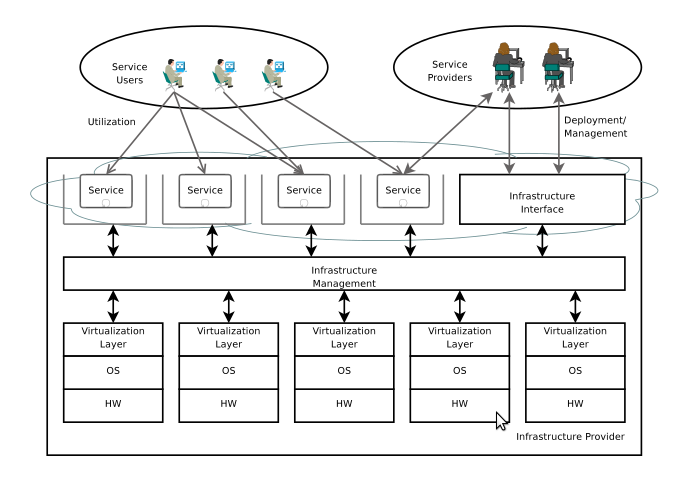
\includegraphics[width=\linewidth]{cloud_actors}
    \caption{Cloud Actors~\cite{Buyya2009599}.}
    \label{fig:cloud_actors}
  \end{center}
\end{figure}

\textbf{The actors:}\\
Service Providers make services accessible to Service Users through Internet-based Interfaces. The computing infrastructure is offered “as a service” by the Infrastructure Providers, moving computing resources from the SPs to the IPs, in order to give the firsts flexibility and reduced costs.

\textbf{The scenarios:}
\begin{itemize}
\item Infrastructure as a Service – IPs are responsible for the management of a large set of computing resources, such as storing and processing capacity. If they use virtualization, they can split, assign and dynamically resize the resources to build ad-hoc systems as the customers (SPs) demand, by deploying the software stacks that run their services.
\item Platform as a Service – Clouds offer an additional abstraction layer – they can provide the software platform where systems run on. The sizing of the hardware resources demanded by the execution of the services is made in a transparent manner. The applications developed are run on the provider's infrastructure and are delivered through the Internet from the provider's servers. The Google Apps Engine is a very good example.
\item Software as a Service – Cloud systems can host many services that users can be interested in, such as online word processors or even Google Apps. \cite{knorr,vaquero}
\end{itemize}

In the article written by Vaquero et al, many Cloud definitions are gathered. Markus Klems states that the key elements for the Cloud are immediate scalability and the optimization of resources usage, these being bring provided by increased monitoring and automation of resources management. Jeff Kaplan and Reuven Cohen prefer to focus on the business model, paying more attention to the collaboration and pay-as-you-go and reducing the costs of investment. Douglas Gourlay and Kirill Sheynkman define the Cloud as being simple virtualized hardware and software, combined with monitoring and provisioning technologies. \cite{21experts,vaquero}

McFedries believes that the basic unit of the Cloud is nothing other than data centers - huge collection of clusters - that can offer a large supply of computing power and storage simply by using whatever resources they can spare.\cite{ieees}

Kevin Hartig defines Cloud Computing as being able to access resources and services needed to perform certain tasks with needs that are constantly changing. The application or user requests access from the cloud rather than on a specific endpoint of the network or a resource. The Cloud becomes a virtualization of resources that is both self maintainable and manageable, a view also shared by Jan Pritzker, who focuses his definition on virtualization and on-demand resource allocation. Other authors such as Reuven Cohen, Praising Gaw, Damon Edwards and Ben Kepes (to name a few) are strong believers that Cloud computing is nothing more other than a buzz word, grouping concepts such as deployment, load balancing, provisioning and data and processing outsourcing.\cite{21experts}

Having this in mind, Vaquero et al believe that the Cloud is a large pool of easily usable and accessible virtualized resources (such as hardware, development platforms and/or services), these being dynamically reconfigured to adjust to a variable load (scaling) also allowing for an optimum resource utilization. The pool of resources is typically exploited by a pay-per-use model in which guarantees are offered by the Infrastructure Provider by means of customized Service-Level Agreements. The authors also state the set of features that resemble this minimum definition would be scalability, pay-per-use utility model and virtualization. \cite{vaquero}

Brian Hayes states in his article that even though the future of Cloud computing is still unclear, there are a few directions in which it can go. One of those directions is Web based services, such as Google Docs or even Photoshop Express. Salesforce.com also offers a variety of online applications and its slogan is actually "No software!". 

As mentioned earlier in the report, Amazon.com also ventured into this new paradigm, offering data storage and computing capacity, each of these services being able to expand and contract as the users need (elasticity) and Google has its App Engine, providing hosting on Google server farms.

There is great concern in terms of scalability in the Cloud, as it might be necessary to organize resources so that the program runs flawlessly even though the number of concurrent users increases might arise. Hayes also mentions that Cloud computing raises questions in terms of privacy, security and reliability, since personal documents are being delivered to a third-party service.\cite{hayes}

Nicholas Carr writes in his book that a shift is happening, where the Cloud is becoming similar (if not equal) to the electric grid, as we can connect to the Cloud and get data, storage space and processing power cheaply and instantly (Utility Computing). \cite{carr}

Aaron Weiss writes in his article that the Cloud is robust, even self-healing, as it has many sources from where to get the power to recover from whatever accident occurs. Weiss states that the Cloud is also very power consuming, as roughly 50 percent of the energy it consumes comes from the cooling process alone. Giants such as IBM and Microsoft are also scouting locations where the hydroelectric power is cheaper and greener, so they can establish their cluster centers.\cite{aaron-clouds}

\subsection{Utility Computing} \label{utility}

Computing is going in such a direction that the services that are made available to the user are being done in such a way that computing is becoming equal to traditional utilities such as water, gas, electricity and telephone services.\cite{Buyya2009599}

In an article published by InfoWorld (formerly the Intelligent Machines Journal), Utility computing is mentioned as being a form of Cloud computing, where storage and virtual servers are being offered and can be accessed on demand, such as the services offered by Amazon.com, Sun or IBM. \cite{grids-and-clouds}

IBM Global Services provide the following definition for Utility Computing:

\begin{quote}
``Utility computing is the on demand delivery of infrastructure, applications, and business processes in a security-rich, shared, scalable, and standards-based computer environment over the Internet for a fee. Customers will tap into IT\footnote{Information Technologies} resources - and pay for them - as easily as they now get their electricity and water.''~\cite{ibm-utility}
\end{quote}

Utilities have the following characteristics:
\begin{itemize}
\item Necessity - Users depend on utility services to fulfill their day-to-day needs. It takes time for distribution networks to spread and costs to decline, as it also takes time for users to adapt to the service. Once they do, the service may grow in importance as users begin to find new ways to reap benefits from it;
\item Reliability - The service must be readily available when and where the user requires it, as a temporal or intermittent loss of service may cause several issues to the user. Redundancy must be built into production capacity in order to make up for hypothetical service failures;
\item Usability - Users have a ``plug-and-play'' mentality and they need to feel at ease with whatever feature they are using;
\item Utilization rates - Utilities are driven by a necessity to carefully manage utilization rates. User demands for utility serves mays vary over time and across service regions. This may lead to spikes in utilization of the service and under-utilization in off-peak periods. Service providers must have in mind that how the service is billed may influence how users use that service;
\item Scalability - As production capacity grows, the unit cost of production shrinks. It might be expected that as the demand for the service rises, the quality of service may decline or vice-versa~\cite{ibm-utility}.
\end{itemize}

Bhattacharya and Vashistha state that utility based computing allows computing resources to be available for a customer on demand, as the customers subscribe to the services of the utility provider and only pay for the quantum of the resources used. This allows any customer to cut down on IT infrastructure spendings as they can simply subscribe to the provider's services and use the computing resources at will, only paying for as much as they use. Typical measures of usage include metered CPU hours and memory space usage~\cite{bhatta-utility}.

Ross and Westerman write in their article that utility computing relies on several important technical capabilities to deliver what it promises - services available on-demand. The authors believe that for most firms, the impact of utility computing will be on the extent and nature of outsourcing. The benefits that can be obtained only enhance the current benefits of IT and business processes outsourcing: lower cost, variable capacity and increased strategic focus. On demand capacity leads to firms to invest less in computing capacity. Advances in autonomic computing may reduce the number of people needed to monitor operations and thus reduce labor costs.

The authors believe that firms will be able to do more with less and will be able to allocate their most strategic resources to their most strategic opportunities~\cite{ross}.

\section{Grids VS. Clouds} \label{sec:gridsvsclouds}

As one knows, Grids and Clouds share a few goals, such as reducing computing costs and increasing flexibility and reliability through the use of third-party operated hardware.

Vaquero et al lay out a very comprehensive list of features and discuss the similarities and differences between them. The list includes resource sharing, heterogeneity, virtualization, security, the offer of high level services such as metadata search, the awareness of architecture, dependencies and platform, software workflow, scalability and self management, standardization, payment model and quality of service. The list is shown in Figure~\ref{fig:grids_vs_clouds} which is in Appendix~\ref{chap:ap1}.

The authors also believe that Grids are meant to be user friendly, virtualized and automatically scalable utilities, something that steps into the Clouds’ path, but they still need to be able to incorporate virtualization techniques in order to obtain some advantages already present in the use of Clouds, like migrability and hardware level scalability.\cite{vaquero}

A few members of the Enabling Grids for E-sciencE (EGEE, now part of the European Grid Infrastructure) performed a comparative analysis on Grids and Clouds, focusing two implementations of both: the EGEE project for Grid and the \textit{Amazon Web Service} (AWS) for Cloud, using metrics such as performance, scale, ease of use, costs and functionality, amongst others. The Grid in use by the EGEE runs on gLite, an open source software which had development funding from the EGEE, described in a later section of this document, as it is used in some extent by FEUP's cluster system.

When comparing both EGEE Grid and the \textit{Amazon Web Service}, the authors of the analysis encounter a set of differences and similarities:
\begin{itemize}
\item The AWS does not expose how they operate their data centers and how they implement the user interfaces, execute the user requests and maintain their accounting, its back-end is still a grey area;
\item The EGEE Grid exposes both user interface as well as the resource interface to permit providers to connect their resources. The AWS hides this second interface;
\item The authors assume that on the resource side, both systems work in similar manner, as both cases require a queueing mechanism whether the data center is dispatching a grid job via a batch system or is requested to instantiate a new virtual machine;
\item The greatest benefit of the Cloud proposed by Amazon is its interfaces and usage patterns, focused on simplicity;
\item Both services are not fail-proof, but the authors consider that a centralized Cloud might not be able to provide the resilience that the distributed nature of EGEE does;
\item Grids are typically used for job execution - limited duration execution of a program, part of a larger set of jobs, consuming or producing a significant amount of data. Clouds, even though they support a job usage pattern, they seem to be more often used for long-serving services;
\item Amazon bills users for computing resources usage with a minimum of one hour usage. This stops being efficient when dealing with a large number of small jobs;
\item Elasticity in the Grid is made by adding worker nodes at a site or adding new sites;
\item The complexity in the Cloud is kept server-side, which makes its entry point very low, something that is still considered a goal to achieve for Grids. \cite{grids-and-clouds}
\end{itemize}


\section{Technology Review}\label{sec:developments-apps-services}

With the shift of the computing industry towards a provision of Platform as Service and Software as a Service, consumers can access resources on-demand without having to preoccupy themselves with time and location, Buyya et al believe that there will be an increasing number of Cloud platforms being developed~\cite{Buyya2009599}. Two of those platforms are \textit{OpenNebula} and \textit{OpenStack}, open-source toolkits for Cloud management. In this report they will both be analyzed, but as they play a major role in this project, they were given their own section in this chapter (\ref{sec:stack-nebula}).

\textit{Amazon}'s computing service (\ref{aws}), \textit{Google's App Engine} (\ref{googleapps}) and \textit{Microsoft Azure} (\ref{azure}) are described in this section.

\subsection{AWS - Amazon Web Services}\label{aws}

The \textit{Amazon Web Services} consist of several components, but only two will be taken into consideration in this document, as they are the most relevant to the work discussed: \textit{Amazon's Simple Storage System} (\ref{amazon-sss}) and \textit{Amazon's Elastic Computing Cloud} (\ref{amazon-ec}).

\subsubsection{Amazon's Simple Storage Service}\label{amazon-sss}

The core service for the \textit{Amazon Web Services} is the \textit{Amazon's Simple Storage Service}, that gives the user the power to store large amounts of data in a reliable way which does not hinder its availability. Data is accessed through protocols such as SOAP\footnote{Simple Object Access Protocol - Used to exchange information in the implementation of Web Services in computer networks.} and REST\footnote{Representational State Transfer - Style of software architecture for distributed hypermedia such as the World Wide Web.}, while also being able to be accessible via normal web browsers.
The storage model runs on a two-level hierarchy, where the users can create \textit{buckets} and place data \textit{objects} in those buckets. Strings are used as keys for both buckets and objects, thus being able to be easily incorporated in URLs. Users are charged 15 US cents per Gigabyte per month, each user being able to have up to 100 buckets and each can hold up to 5GB of data.\cite{hazel}

\subsubsection{Amazon's Elastic Computing Cloud}\label{amazon-ec}

Physically speaking, the \textit{Elastic Computing Cloud} (EC2) is a large number of computers on which Amazon provides time to paying customers, these computers being spread all over the United States. EC2 is based on the XEN virtualization technology, which allows one physical computer to be shared by several virtual ones, each with its own operating system.

Through the use of virtualization, the users create an image of their software environment using the tools provided. This will be used to create and instance of a machine in Amazon's Cloud. Customers can freely choose configuration templates for their instance and they can create and destroy the instances at will, enabling the software to scale itself to the amount of computing power it needs.\cite{grids-and-clouds, hazel}

Amazon has released \textit{Elastic IPs} (Static IPs for Dynamic Cloud Computing), which allows the assignment of static IPs to dynamic resources that are deployed via EC2, as well a service that enables users to request EC2 instances to be geographically distributed, as a response to the demand for EC2 IP addresses in a static range for application range for applications like email service hosting, as well as providing a safety net in case the operations of an Amazon Web Services data center go awry. 

Amazon provides a variety of ways of requesting the EC2 instances, namely through the use of Web Services, supporting Buyya et al's Cloud definition previously mentioned in the document.

Amazon has also introduced its own performance unit named "EC2 Compute Unit". Since Amazon ventured into the Utility computing field, model it follows differs from the traditional way developers were formatted to think about CPU resources. Instead of renting a certain processor for several months or years, it is now rented by the hour. One EC2 Compute Unit provides the CPU equivalent of a 1.0-1.2 GHz 2007 Opteron or 2007 Xeon processor.\cite{amazon-aws}

\subsection{Google Cloud - Google's App Engine}\label{googleapps}

The \textit{Google Cloud}'s official name is \textit{App Engine} or \textit{Appengine}. It gives developers the ability to run web applications on Google's infrastructure, the same that is being used by \textit{Google} for \textit{GMail} and \textit{Google Docs}.
The Cloud appears to be a platform accessible over the Internet with limitless hardware, the latest software and abundant storage for deploying web applications.
The \textit{App Engine} has the following features:
\begin{itemize}
\item Automatic horizontal scaling and load balancing;
\item APIs\footnote{Application Programming Interface} for authenticating users with Google Accounts and for sending emails. No system administration is needed by the user to set up or allow access to these APIs;
\item Fully featured Eclipse developed environment that simulates \textit{Google App Engine} on the localhost for development and testing;
\item Persistent storage and support for transactions and queries using the standard JDO\footnote{Java Data Objects} and JPA\footnote{Java Persistence API} APIs;
\item Generous free quotas, which allow small universities to have access to the same hardware and software as large industries. Each user can have 10 applications created, each with 10 versions, which totals an effective development environment of 100 applications. A free account supports six and a half CPU hours a day, with 1GB of stored data and sending email to 2000 recipients a day and a max of 5 million page views a month;
\item It is free, with no contracts to sign, no hardware expense and no system administration costs for maintaining, updating, patching or backing up \textit{App Engine};
\item Eclipse plug-in available for Apple, Linux and Windows, which allows standard debugging using Eclipse debug tools. It provides menu based functionality to automatically upload the application to the Google App Engine;
\item Requires no system administration;
\item Simple web based, user friendly console.\cite{googleapp}
\end{itemize} 

\subsection{Microsoft Azure}\label{azure}

\textit{Microsoft Azure} platform is a cloud computing platform which offers a set of cloud computing services similar to those offered by Amazon Web Services. \textit{Windows Azure Compute} (Microsoft's counterpart to Amazon's EC2), only supports Windows virtual machines and offers a limited variety of instance types when compared with Amazon's EC2. Its instance type configurations and cost scales up linearly from small to extra large and its instances are available in 64 bit x86\_64 environments. 

It has been speculated that the clock speed of a single CPU core in \textit{Azure}'s terminology is approximately 1.5 GHz to 1.7 GHz.\cite{azure-paper}
Windows Azure enables developers to build, host and scale applications in Microsoft datacenters, not requiring upfront expenses, long term commitment and users only pay for the resources they use. 
Windows Azure relieves the user from the effort of configuring load balancing and failover, is designed to let developers build applications that are continuously available, even if they need software updates and hardware failures occur.\cite{azure}

\section{FEUP's Computing System}\label{feup}

In this section FEUP's computing system is analyzed in detail. The cluster system and the technologies it uses in its management are described and detailed. FEUP's cluster system currently uses three different technologies, \textit{Moab}, \textit{gLite} and \textit{Condor}.
Currently FEUP currently has both \textit{OpenNebula} and \textit{OpenStack} running (the last one for research purposes only), both technologies having been already discussed in the previous section(~\ref{sec:stack-nebula})


\subsection{Clusters}\label{clusters}

Three different technologies are currently in use by FEUP's Cluster system: \textit{Moab}(\ref{moab}), \textit{gLite}(\ref{glite}) and \textit{Condor}(\ref{condor}).

\subsubsection{Moab Cluster Suite}\label{moab}

\textit{Moab Cluster Suite} is a proprietary tool for high performance computing systems, developed by the company \textit{Cluster Resources}. It has built-in modules for work management, Cluster administration and monitoring, report creation. It is composed by three essential components:
\begin{itemize}
\item \textbf{Moab Workload Manager} - scheduling and workload management engine;
\item \textbf{Moab Cluster Manager} - graphical interface for Cluster administration, monitoring and report analysis;
\item \textbf{Moab Access Portal} - web based portal for job management and submission, directly focused on the end-user.
\end{itemize}

A resource manager supplies the system with basic functionalities for initiating, stopping, canceling or monitoring jobs. \textit{Moab Workload Manager} uses a resource manager's services to get information about the state of the resources and the node workload. It is also used to manage jobs and to send information on how they should be run and it can be configured to manage more than one resource manager simultaneously.
Its composing nodes can be split into three groups:
\begin{enumerate}
\item \textbf{Master node} - Manages the resources;
\item \textbf{Submissive/Interactive nodes} - Allow users to manage and submit jobs into the system;
\item \textbf{Computing nodes} - Execute the submitted jobs.
\end{enumerate}

Is is also possible to split the nodes into two groups - source and destination nodes. The first ones are the nodes where there users, portals or other systems can submit their jobs and the latter ones are where the jobs are executed. Jobs originate in a source node and are transferred to the destination nodes. Decisions are made in the source nodes, so it is possible to choose which nodes will execute the submitted jobs.
Moab also allows for the establishment of connections between several Grid systems, which permit access to additional resources.\cite{jorge-ruao, moab}

\subsubsection{gLite}\label{glite}

\textit{gLite} consists in a set of components designed with the objective of building a Grid computing infrastructure for resource sharing developed by the project EGEE (Enabling Grids for E-sciencE), also mentioned in an earlier section.
\textit{gLite} is based on four core concepts:
\begin{itemize}
\item \textbf{Computing Element (CE)} - Set of local computational resources, namely a Cluster. It is composed by three components:
	\begin{itemize}
	\item \textbf{Grid Gate} - generic interface for the Cluster who receives jobs and submits it to the Local Resource Management System (LRMS);
	\item \textbf{Local Resource Management System (LRMS)} - Sends the jobs to the worker nodes for execution;
	\item \textbf{Worker Nodes} - Cluster nodes where jobs are executed.
	\end{itemize}
\item \textbf{Storage Element (SE)} - Supplies access to data storage resources;
\item \textbf{Information Service (IS)} - Resource research is made through this component, which is also responsible for supplying information regarding resources and their state;
\item \textbf{Workload Management System (WMS)} - Receives jobs from users, appropriately allocates a CE, saves jobs states and gets the final results.\cite{jorge-ruao,glite}
\end{itemize}

\subsubsection{Condor}\label{condor}

\textit{Condor} is a free and open-source workload management system, developed by the \textit{Condor Research Project}.
It has built-in job queueing mechanisms, scheduling and priority policies, resource monitoring and management. Users submit jobs to \textit{Condor}, which puts them in a queue, chooses when and where to execute them based on defined policies, carefully monitors their progress and informs the user when the jobs are finished.
\textit{Condor} can manage dedicated nodes or harness the CPU energy wasted in workstations that are turned on but unused. If the system detects the machine became suddenly unavailable, \textit{Condor} can migrate the state of the job into a different machine and resume work. 
It offers an extremely flexible structure to assign resources to jobs, allowing these to have specific requisites and resource preferences, as well as enabling the resources to specify preferences over jobs to execute.
Each machine from \textit{Condor} can play several roles:
\begin{itemize}
\item Central Manager - Machine that collects information and makes the negotiation between resources and resource requests. All resource requests go through the \textit{Central Manager}. There can only be one \textit{Central Manager} in a \textit{Condor} infrastructure;
\item Execute - Machine which executes jobs, therefore allowing the network to take advantage of its resources. Any machine can be configured to take this role;
\item Submit - Machine responsible for the job reception and submission to the \textit{Central Manager}. Any machine can be configured to take this role;
\item Checkpoint Server - Machine which stores checkpoint files for all submitted jobs.\cite{jorge-ruao,condor}
\end{itemize}


\section{Cloud Creation and Management Software}\label{sec:stack-nebula}

As mentioned in the previous section (\ref{sec:developments-apps-services}), \textit{OpenStack} and \textit{OpenNebula} are two projects that deserve their own section when talking about the developments, applications and services that exist in their field. 

Since the objectives of the project involved the implementation of a virtual environment creator and manager, both these platforms were deemed worthy of a more detailed inspection. Both projects are open source (\textit{OpenNebula} offers an ``Enterprise Edition'', which can put its open source status in question~\ref{subsec:opennebula}) and one of them will run alongside the web page that will be developed and will interact with.

Image contextualization will be approached, since it is directly linked to one of the objectives of this project --- creating different virtual environments according to the users' needs.

Project \textit{Aeolus} will also be discussed in this section, as it contains one of the tools that will be discussed in the next section (~\nameref{sec:iso}) and is related to the objective refered earlier, \nameref{subsec:oz}.

\subsection{OpenStack}\label{subsec:openstack}

\textit{OpenStack} is a global collaboration of developers and cloud computing technologists producing the open source cloud computing platform for public and private clouds. The aim of this project is to deliver solutions for all types of clouds by being simple to implement, massively scalable and filled with features. 

First released in October 2010 and now on its fifth version (codename Essex), OpenStack has undergone major changes and revamps over the past months ~\cite{openstack}.

It was founded by \textit{Rackspace Hosting} and NASA\footnote{North American Space Agency} (deployed as NASA's Nebula cloud~\cite{nasa-nebula})and it has grown to be a global software community of developers collaborating on a standard open source cloud operating system. Current companies involved with \textit{OpenStack} include \textit{OpenStack Foundation}, \textit{Canonical}, \textit{Cisco}, \textit{Dell}, \textit{Red Hat}, \textit{SUSE} and \textit{Yahoo!}. \cite{stackgithub}

\textit{OpenStack}'s mission is to enable any organization to create and offer cloud computing services running on standard hardware.

All of its code is available under the \textit{Apache} 2.0 license and as such, anyone can run it, build applications on it or submit changes back to the project. It is commoditizing the IaaS market, enabling the users to get from \textit{Amazon} today into their own private data centers and cloud environments by using open source. \cite{stackgithub}

\subsubsection{OpenStack Architecture}\label{subsubsec:openstack_arch}
  
The following figure depicts OpenStack's software diagram:

\begin{figure}[h]
  \begin{center}
    \leavevmode
    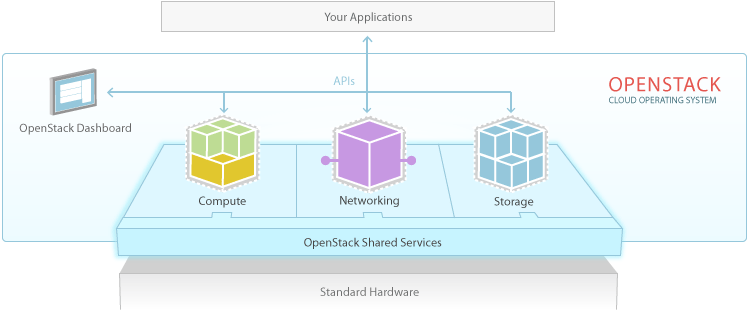
\includegraphics[width=\textwidth]{openstack-software-diagram}
    \caption{OpenStack Software Diagram\cite{openstack}.}
    \label{fig:openstack_sw_diag}
  \end{center}
\end{figure}

\textit{OpenStack} has four major components:

\begin{itemize}
\item \textbf{Compute} - Also known as \textit{Nova}, it is designed to provision and manage large networks of virtual machines. Provides an API so that developers who wish to build cloud applications can access the compute resources, as well as web interfaces for administrators and users. Its architecture is designed to be flexible in the cloud design, so that no proprietary hardware or software is required and has the ability to integrate with legacy systems and third party technologies. \textit{Nova} can manage and automate pools of compute resources and works with a great deal of virtualization technologies, enabling the administrators to use multiple hypervisors, such as KVM or XenServer.
\item \textbf{Networking} - A pluggable, scalable and API-driven system for managing networks and IP addresses. Keeps the network from bottlenecking or being a limitation factor in the cloud deployment. Designed to provide flexible networking models to cater the needs of different applications and user groups. Manages IP addresses, allowing both static IPs or DHCP. Allows the administrator or the user to reroute traffic in case of maintenance or failure. \textit{OpenStack Networking} has an extension framework which allows extra network services, such as intrusion detection systems, firewalls and VPNs to be deployed and managed.
\item \textbf{Storage} - Also known as \textit{Swift}, it is ideal for cost effective and scale-out storage~\footnote{A storage system that uses a scaling methodology in order to create a dynamic storage environment which will support balanced data growth on an as-needed basis. Its architecture uses a number of storage nods that are configured to create a storage pool or are configured to increase computing power and is designed to scale boyth capacity and performance~\cite{scaleout}}. It has a fully distributed and API-accessible storage platform which can be integrated directly into applications or used as a backup, achiving and data retention tool. It allows for block devices to be exposed and connected to compute instances for expanded storage, better performance and integration with enterprise storage platforms. \textit{OpenStack Swift}'s object storage is a distributed storage system for static data such as VM images, photo and email storage, backups and archives. It has no central point of control thus providing greater scalability, redunndancy and durability. Storage clusters can scale horizontally by adding new servers. If one of the servers or a hard drive fails, OpenStack replicates its content from other active nodes to a new location in the cluster. Furthermore, \textit{OpenStack} uses algorithms in order to replicate and distribute data accross different devices which allows for the use of inexpensive hard drives and servers.
\item \textbf{OpenStack Dashboard} - Also known as \textit{Horizon}, it provides administrators and users with a GUI to access, provision and automate cloud-based resources. It is extensible, making it easy to attach third party services, such as billing, monitoring and additional management tools. It is a simpler way to access the resources, which can also be done by building their own tools using either \textit{OpenStack}'s or EC2' compatible API.
\end{itemize}

Alongside the four components described above, \textit{OpenStack} also has a few shared services which make implementing and controlling the cloud an easier job. They are designed in a way that they can integrate with themselves as well as the components above.

\textit{OpenStack} has its own identity service - named \textit{Keystone} - which shows a central directory of users mapped to the \textit{OpenStack} services they can access. \textit{Keystone} acts as a common authentication system accross the operating system that the cloud sits on and can integrate with existing backend services such as LDAP. This identity service allows the administrator to configure centralized policies accross the users and systems as well as defining permissions for the four major components depicted above, whereas the users can get a list of services they can access, make API requests or log into the web dashboard - \textit{Horizon} - to create resources linked to their account.

Another important serviced provided by \textit{OpenStack} is its image service \textit{Glance}. It provides discovery, registration and delivery services for disk and server images. It has the ability to snapshot a server image and store it, which can then be used as a template to get new servers up and running very quickly - and consitently in the case of setting up multiple servers - rather than installing a server OS and individually configuring the additional services required. \textit{Glance} can store both disk and server images in a great variety of backends, including \textit{OpenStack}'s own object storage. A standard REST interface is provided for querying information on disk images and that lets clients stream the images to new servers. The image registry supports a wide range of formats, which include images generated by KVM, Qemu, VMWARE and RAW images.

This project is under close surveillance by CICA as it is viewed as a possible substitute for \textit{OpenNebula}. \textit{OpenStack} is also discussed in the following chapter~\ref{chap:chap3} as it is one of the focus points of the work realized.

\subsubsection{DevStack}\label{subsubsec:devstack}

Since \textit{OpenStack} still has a somewhat complex deployment process, \textit{DevStack} was created in order to provide whoever wishes to try out \textit{OpenStack} for development purposes.

It is essentially a set of scripts and utilities to quickly deploy an \textit{OpenStack} cloud.
 
Its goals include the following:
\begin{itemize}
\item To enable the user to quickly build dev \textit{OpenStack} environments in a clean Ubuntu or Fedora environment;
\item To describe working configurations of \textit{OpenStack}; 
\item To make it easier for developers to get familiar with \textit{OpenStack} without the need to understand every single part of the system at once.
\end{itemize}


Created by \textit{Rackspace Cloud Builders}~\footnote{Business launched by \textit{Rackspace} that helps other businesses deploy \textit{OpenStack}~\cite{cloudbuilders}}, \textit{DevStack} will be used as it simplifies the deployment process (and is used by FEUP's \textit{OpenStack} researcher). \textit{DevStack} will be further expanded in Chapter~\ref{chap:chap3}, when its deployment is discussed.

\subsection{OpenNebula}\label{subsec:opennebula}


\textit{OpenNebula} was initially created as a research project in 2005 by Ignacio M. Llorente and Rubén S. Montero from \textit{Universidad Complutense Madrid}, being publicly released in 2008. It now works as an open source project after having evolved through several releases (now on version 3.4). It is the result of many years of research and development in efficient and scalable management of virtual machines on large-scale distributed infrastructures in close collaboration with \textit{OpenNebula}'s user community and leading experts in cloud computing. 

Most of \textit{OpenNebula}'s features have been developed as a response to the use cases from many of the companies involved in the project (these include RESERVOIR~\footnote{\textit{Framework} developed to aid both techonology and information specialists in enterprises in creating a cloud with all the coding and architecture specifications needed.~\cite{reservoir}}, \textit{StratusLab}~\footnote{A project aiming to develop a complete and open-source cloud distribution that allows both grid and non-grid resource centers to offer and exploit an IaaS cloud. It is particularly focused on enhancing distributed computing infrastructures such as the European Grid Infrastructure (EGI)~\cite{stratuslab}} and \textit{4CaaSt}~\footnote{Project created for the development of an advanced PaaS cloud platform which supports the optimized and elastic hosting of Internet-scale multitier applications, embedding all the necessary features, so that the programming of rich applications is simplified.~\cite{4caast}}) and its technology has evolved mostly thanks to the effort the community has put into it.~\cite{opennebula}

It was first released as a software package in \textit{Ubuntu} 9.04, has its own command-line tools and gives the user different configuration scripts which enable a simple and flexible way to design and manage running virtual machines. Since the release of version 3.0, \textit{OpenNebula} has introduced a GUI called \textit{Sunstone} (only runs on \textit{Firefox} and \textit{Chrome} browsers), which allow the users and administrators to manage all \textit{OpenNebula}'s resources (as long as they have access to them, something that can be regulated via ACLs or external modules)~\cite{jorge-ruao}.

\textit{OpenNebula}'s architecture is presented in Figure~\ref{fig:nebula_arch} and its main components are presented in Figure~\ref{fig:nebula_components}.

\begin{figure}[h!]
  \begin{center}
    \leavevmode
    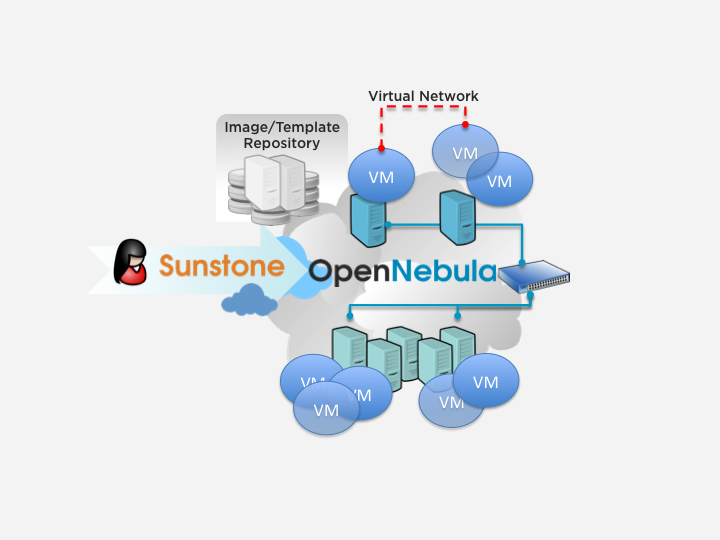
\includegraphics[scale=0.5]{nebula_arch}
    \caption{OpenNebula's Architecture~\cite{nebulatech}.}
    \label{fig:nebula_arch}
  \end{center}
\end{figure}

\begin{figure}[h!]
  \begin{center}
    \leavevmode
    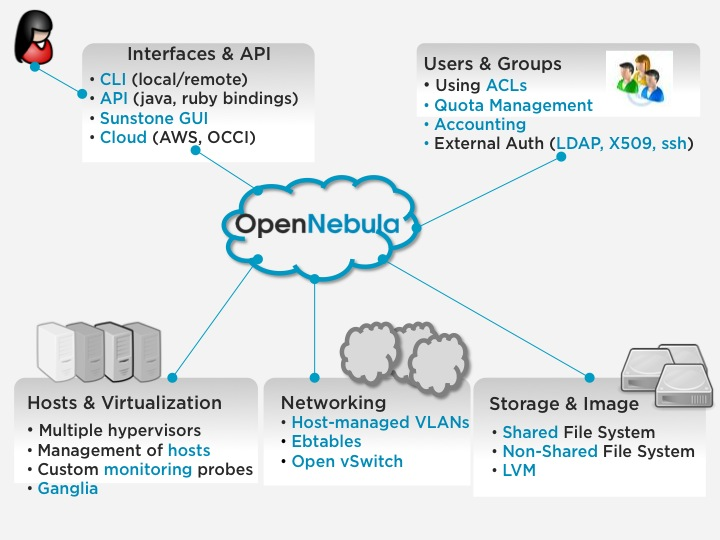
\includegraphics[scale=0.5]{nebula_components}
    \caption{OpenNebula's components~\cite{nebulacomponents}.}
    \label{fig:nebula_components}
  \end{center} 
\end{figure}


\begin{itemize}
\item \textbf{Interfaces and APIs} --- \textit{OpenNebula} offers two main ways to manage its instances: CLI or GUI (\textit{Sunstone}). Several cloud interfaces such as \textit{OCCI}~\footnote{Open Cloud Computing Interface. Web service that enables the user to launch and manage virtual machines in the \textit{OpenNebula} installation.~\cite{occi}} and EC2 Query~\footnote{Web service that enables the use of virtual machines through Amazon's EC2 Query Interface (\ref{amazon-ec})};
\item \textbf{Users and Groups} --- \textit{OpenNebula} supports user accounts and groups, as well as several authentication and authorization mechanisms. These can be used to create isolated compartments inside the same cloud (multi-tenancy). An ACL mechanist also exists to allow different role management;
\item \textbf{Hosts} --- Various hypervisors are supported by the virtualization manager, which has the ability to control and monitor the lifecycle of VMs, something that can be extended to the physical hosts. It is compatible with Xen, KVM and VMware, three \textit{platform virtual machines} that emulate the whole physical computer machine;
\item \textbf{Networking} --- A network subsystem that allows \textit{OpenNebula} to easily integrate with specific network requirements of existing datacenters;
\item \textbf{Storage} --- \textit{OpenNebula} supports multiple data stores in its storage subsystem which provides extreme flexibility in planning the storage backend. Disk images can be stored in both file and block device, also having support for the VMware datastore;
\item \textbf{Clusters} --- Clusters are pools of hosts that share datastores and virtual networks. They are used for load balancing, high availability and high performance computing.
\end{itemize}
\textit{OpenNebula} does not have a built-in utility to create VMs from scratch, but its templates allow the VMs to boot an ISO image, leaving the user with just creating an empty hard disk image.

It provides monitoring capabilities which become rather useful when there is a need to troubleshoot, scale or control resource allocation scenarios. \textit{OpenNebula} exports drivers that communicate directly with the hypervisor (KVM - \ref{hyper}) and return useful data, such as the amount of CPU used, reserved and used memory and network traffic.\cite{open-clouds}

In March 2010, \textit{OpenNebula}'s main authors founded \textit{C12G Labs}~\footnote{Company that provides enterprise-grade solutions built around \textit{OpenNebula}}, which has led to it being referred to as "...proprietary tech with an element of openness...", which could limit its growth.~\cite{linkedin-opennebula}

\subsection{Project Aeolus}\label{subsec:aeolus}

\textit{Aeolus} consists of a set of tools to build and manage groups of VMs across clouds (both public and private). It has four components:

\begin{itemize}
\item \textbf{Conductor} --- Provides cloud resources to users, manages their access to and use of those resources, controls user's instances in clouds, launches a VM on a cloud, keeps track of it during its lifecycle and cleans up after the VM is no longer needed. It alerts the user when something happens, such as the VM crashing or the user is about to exhaust the hours of monthly usage, for example. It instructs the user on which cloud to chose depending on certain parameters, including cost, quality of service (QOS) data and other metrics. If the user wishes to, the Conductor can perform that choice;
\item \textbf{Composer} --- Builds cloud-specific images from generic templates, in order to allow users to choose clouds freely by using compatible images. The user can specify arguments to pass into the build process so that the software installation can be configured. Images can be rebuilt from the original template in order to update packages or for feature enhancements, bug fixes or security issues.
\item \textbf{Orchestrator} --- Manages groups of instances. Users can automatically bring up a set of different instances on a single cloud or group of clouds, configure them and make them aware of each other;
\item \textbf{HA Manager} --- Makes instances or groups of instances manageable. Provides isolation, recovery and notification of failed applications or instances. Lets the user create policies for maintaining or relaunching services within a specific infrastructure.
\end{itemize}

\subsection{Contextualization}

At the end of instantiating a VM, its data can be set or overrun by user request, thus creating the possibility of setting up an infinite number of environments using only one VM image.

\textit{OpenStack} and \textit{OpenNebula} have different ways of handling this process, which are described in this section of the document.

\subsubsection{\textit{OpenStack}}

\textit{OpenStack}'s \textit{Image Service} provides discovery, registration and delivery services for disk and server images, taking advantage of \textit{OpenStack}'s ability to copy or snapshot a server image and store it immediately~\ref{subsubsec:openstack_arch}.

Currently only \textit{Ubuntu} and \textit{Amazon} AMI images can be contextualized using \textit{OpenStack}. This happens because \textit{cloud-init}~\footnote{\textit{Ubuntu} package that handles early initialization of a cloud instance. It is installed in the \textit{Ubuntu Enterprise Cloud} (UEC) images and also in the official Ubuntu images available on \textit{Amazon}'s EC2.} is used~\ref{essex-cloudinit}.

\textit{cloud-init} handles importing ssh keys for password-less login and setting host name, amongst other things. The instance acquires the instance specific configuration from Nova-compute by connecting to a meta data interface~\ref{essex-cloudinit}.

If an image from a distribution that does not have \textit{cloud-init} is being used, this setup needs to be performed via the use of a set of scripts which should be included in a specific file (rc.local) so they can be executed at boot time.

In Figure~\ref{fig:tiny-flavour} and Figure~\ref{fig:customization-script} the \textit{Horizon} dashboard is shown when launching a new instance. Figure~\ref{fig:customization-script} shows the area where the \textit{cloud-init} configuration file is placed so it can be ran at boot time.

This technology will be used in the solution proposed as it matches perfectly with one of the objectives --- being able to create virtual environments according to the users specifications. \textit{Ubuntu} AMI images will be used as concept proof and to simplify the whole process.

\begin{figure}[h]
  \begin{center}
    \leavevmode
    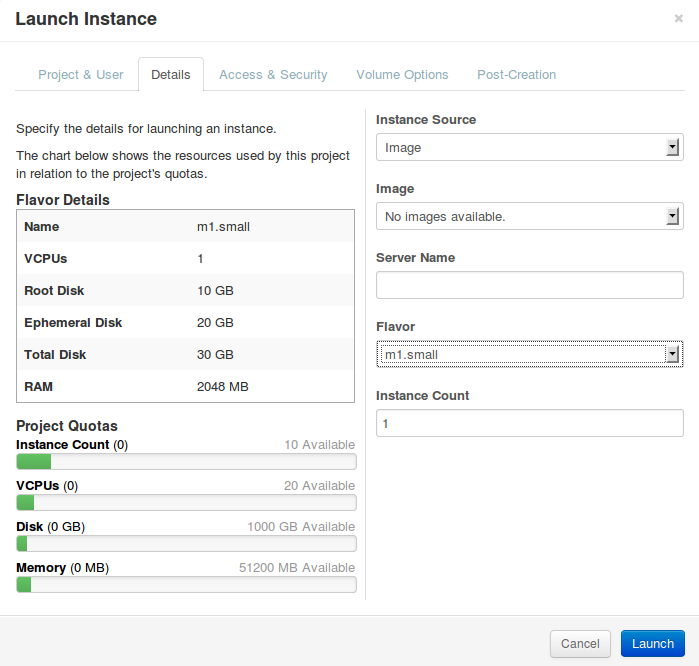
\includegraphics[scale=0.5]{tiny-flavour}
    \caption{Launching an instance in \textit{Horizon}.}
    \label{fig:tiny-flavour}
  \end{center} 
\end{figure}


\begin{figure}[h]
  \begin{center}
    \leavevmode
    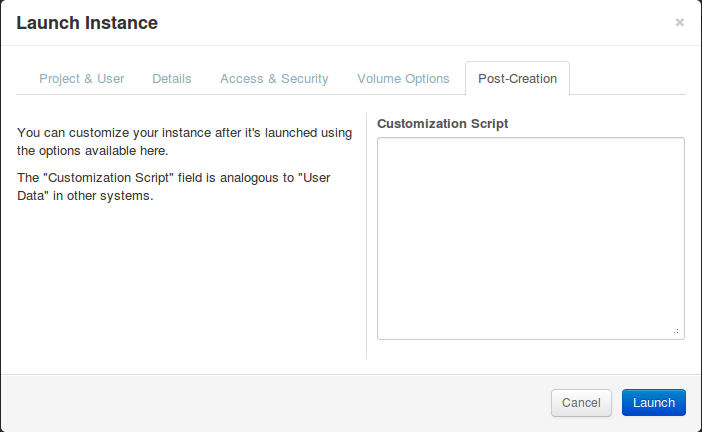
\includegraphics[scale=0.5]{customization-script}
    \caption{Script to be ran once the instance is launched.}
    \label{fig:customization-script}
  \end{center} 
\end{figure}


It is important to mention that information on \textit{cloud-init} was obtained after going on \textit{OpenStack}'s \textit{Internet Relay Chat} (IRC) channel~\footnote{\#openstack on irc.freenode.net} and talking directly to the main contributers of the \textit{cloud-init} module, Joshua Harlow and Scott Moser.

According to both of them, \textit{cloud-init} is in the process of being available to a wider selection of distributions, which include \textit{openSUSE}, \textit{Fedora} and \textit{Red Hat}. 

The conversation is attached in Appendix~\ref{chap:ap3}.

\subsubsection{\textit{OpenNebula}}

As mentioned in section~\ref{subsec:opennebula}, \textit{OpenNebula}'s \textit{Storage System} allows administrators and users to set up images (OS or data) to be be used in VMs. 

\textit{OpenNebula} supports three types of images:

\begin{itemize}
\item \textbf{OS} --- Contains a working operative system;
\item \textbf{CDROM} --- Readonly data;
\item \textbf{DATABLOCK} --- Storage for data, which can be accessed and modificed from different VMs. They can be created from previous existing data, or as an empty drive.
\end{itemize}

The type of an existing image can be changed when performed a specific command and the images can be managed either by using \textit{Sunstone} or \textit{OpenNebula}'s CLI.

In order to create an \textbf{OS Image}, a contextualized VM needs to be created and its disk extracted.
\textit{OpenNebula}- has two contextualization mechanisms available:

\begin{itemize}
\item \textbf{Automatic IP assignment} --- Several pre-created scripts are provided by \textit{OpenNebula} for \textit{Debian}, \textit{Ubuntu}, \textit{CentOS} and \textit{openSUSE} based systems, all of which can be adapted for other distributions.
\item \textbf{Generic Contextualization} --- Configuration parameters are given to a newly started VM by using an ISO image. The VM description file contains the contents of the ISO file (files and directories), instructs the device that the ISO image will become accessible and specifies the configuration parameters that will be written to a file for later use inside the VM.
\end{itemize}

When using the generic contextualization mechanism, the VM description file can be used to create a contextualization image, which will contain the context values. These include the \textit{hostname}, \textit{root} password and the Domain Name Server (DNS). These values will be held inside the CONTEXT parameter residing inside the contextualization image, whose variables can be specified in three different ways:

\begin{itemize}
\item Hardcoded;
\item Using template variables;
\item Pre-defined variables.~\cite{nebula-contextualization}
\end{itemize}

\clearpage
\section{ISO Image creation} \label{sec:iso}

One of the big objectives in this project is the automatic creation of virtual environments. As such, it is necessary to present some of the tools used for this process, having in mind the restrictions enforced by the choices made regarding the rest of the technologies which will be used in the rest of the project, namely \textit{OpenStack} and its restriction regarding the use of \textit{cloud-init} to contextualize the virtual images.

Considering these restrictions, it was chosen to follow the software recommendations made by \textit{OpenStack}'s documentation when building virtual images:

\begin{itemize}
\item \textbf{Oz} --- Part of the \textit{Aeolus} project mentioned in section~\ref{sec:stack-nebula}, it is a command line tool used by \textit{Rackspace Cloudbuilders} to images for Linux distributions;
\item \textbf{VMBuilder} --- \textit{Python} based software package for creating VM images of free software GNU/Linux-based OS. It supports \textit{Xen}, \textit{VirtualBox}, \textit{VMware}, \textit{KVM} and \textit{Amazon EC2}~\cite{vmbuilder};
\item \textbf{VeeWee - Vagrant} --- \textit{VeeWee} being the tool used to easily build \textit{Vagrant}-based boxes or \textit{KVM, Virtual Box} and \textit{Fusion} images~\cite{essex-doc-vms,veewee}.
\end{itemize}

These technologies will be reviewed for further use in the project.

\subsection{Oz}~\label{subsec:oz}

As mentioned earlier, \textit{Oz} is part of a bigger project called \textit{Aeolus}~\footnote{\url{http://aeolusproject.org/index.html}}.

It was created in order to simplify the automaticinstallation of guest OS, akways using the native OS tools to do the installs. This is done so that when when the installation finishes, the disk image left by \textit{Oz} is exactly the same as if was used an installation CD. 

There are three funcionalities available in \textit{Oz}:

\begin{itemize}
\item Install the OS --- \textit{Oz} was built with enough knowledge to install minimal operating systems with little input. It just needs to be told which OS to install and where the installation media is, doing the rest automatically;
\item Customize the OS --- This is the relevant part for the project. \textit{Oz} has the ability to install additional packages and files into the OS;
\item Generate metadata on that OS --- This includes package manifest. This metadata is represented in an XML file denominated ICICLE.
\end{itemize}

In the OS customization process (which is always done as a separate step from the OS install in order to reduce the chances of failure), \textit{Oz} is able to run the native tools, such as \textit{Yum} and \textit{apt-get}; modify the OS disk image in order to allow remote access, start up the OS in a controlled \textit{KVM} guest; run remote commands (for example: \textit{ssh}) to install packages and files and shut down the OS. It then undoes the changes to the disk and generates the metadata on that OS~\ref{oz}.

\subsection{JeOS and vmbuilder}\label{subsec:vmbuilder}

\textit{Ubuntu JeOS} (pronounced ``juice'') is a variant of the \textit{Ubuntu} Server OS, which is configured specifically for virtual appliances. It is no longer available as a CD-ROM ISO for download, but can be built using \textit{Ubuntu}'s \texttt{vmbuilder}. 

\textit{JeOS} is a specialized installation of \textit{Ubuntu Server Editio} with a tuned kernel that only contains the base elements needed to run in a virtualized environment and as such, suitable for the project covered by this document. The tuning is done in order to take advantage of key performance technologies in the virtualization products from \textit{VMware}, creating a combination of reduced size and optimized performance which ensures that \textit{JeOS} delivers a highly efficient use of server resources in a large virtual environment.

With only the minimal required packages and without unnecessary drivers, software companies can configure their OS according to their needs. They have the safety of knowing that the updates required will be limited and the users will be able to deploy virtual appliances on top of \textit{JeOS} which will need less maintenance than what would have been needed were they installed on top of a full server.

\textit{vmbuilder} takes away the need of downloading a \textit{JeOS} ISO. It will fetch the various package and build a VM specifically designed for what the users desire. It is a script that automates the process of creating a ready to use \textit{Linux} based VM, currently supporting the \textit{KVM} and \textit{Xen} hypervisors.

Command line options can be used to perform actions such as adding or removing packages, choosing which \textit{Ubuntu} version and mirror and more.

\textit{vmbuilder} was first introduced as a shell script in \textit{Ubuntu} 8.04 LTS, as a hack to help developers test their code in a VM without needing to restart the server from scratch every time they needed. A few of \textit{Ubuntu} administrators noticed the script, improved and adapted it to so many use cases that the author of this script (Soren Hansen) rewrote it as a \textit{Python} script with revamped goals:

\begin{itemize}
\item Ability to be reused by other distributions other than \textit{Ubuntu};
\item Use plugin mechanisms for all virtualization interactions so that others can easily add logic for other virtualization environments;
\item Provide an easy to maintain web interface as an alternative to the CLI~\ref{jeos}.
\end{itemize}

This technology becomes extremely relevant to the project as it covers the creation of customizable environments.
\subsection{VeeWee and Vagrant}~\label{subsec:veewee}

\textit{Vagrant} is a free and open-source \textit{Ruby} based project, started by Mitchell Hashimoto and John Bender on January 21st, 2010. With its first release on March 7, 2010, \textit{Vagrant}'s goal is to create a tool to manage all the complex parts of development within a virtual environment without affecting the developer's workflow. Its developers are currently working on getting \textit{Vagrant} working on every major OS platform (Linux, OS X and Windows).

\textit{Vagrant}'s development is not supported by any company, as its developers work on the project on their free time. The only external help they get is via contributions, which can be done via completing \textit{Vagrant}'s documentation, its code (open-source project) or submitting financial donations (the developers prefer other types of contributions)~\cite{vagrant-contribution}.

\textit{VeeWee} is a toll built by Patrick Debois as a way to customize the boxes \textit{Vagrant} creates. This process is simple, as \textit{Vagrant} creates three files, one of which is \texttt{definition.rb}, a \textit{Ruby} file which contains the main definition of the template created by \textit{VeeWee}. In this file the user can define settings like the memory and disk size. Another file \textit{VeeWee} creates is \texttt{preseed.cfg} which can be modified to configure the actual install process, controlling details including, but not limited to, the partitions and their size and timezone setup~\ref{vagrant-ducea}.

Besides \textit{Vagrant} boxes, \textit{VeeWee} can be used for:

\begin{itemize}
\item Creating \textit{VMware} and \textit{KVM} VMs;
\item Interacting (creating, destroying, halting and remote accessing them via the \texttt{ssh} command) with those VMs;
\item Exporting those VMs.
\end{itemize}

The customization process relevant to the project by modifying the templates used for creating the images.

\section{Conlusions}\label{sota:concl}

In this chapter the main technologies to consider for the project implementation were presented, as well as some of the key concepts needed for contextualization.
It was decided to use an instance of \textit{Ubuntu JeOS} for the image creation process (with \textit{vmbuilder}) and compare it to the use of \textit{cloud-init} to contextualize an already built (but not contextualized) image.

